% ============================================================
%  Word2Vec para análisis de sentimientos en español
%  Proyecto Final - DS2011 Optimización - UTEC - Grupo 1
%
%  Compilar con:  pdflatex informe_latex.tex   (dos veces)
%  Requiere las figuras en la carpeta results/
% ============================================================
\documentclass[11pt]{article}

\usepackage[utf8]{inputenc}
\usepackage[T1]{fontenc}
\usepackage[spanish,es-tabla]{babel}
\usepackage{amsmath,amssymb}
\usepackage{graphicx}
\usepackage{booktabs}
\usepackage{geometry}
\usepackage{float}
\usepackage{array}
\usepackage{caption}
\usepackage[hidelinks]{hyperref}

\geometry{a4paper,margin=2.5cm}
\graphicspath{{results/}}
\captionsetup{font=small,labelfont=bf}

\newcommand{\sgn}{\operatorname{sgn}}

\title{\textbf{Word2Vec para análisis de sentimientos en español:\\
arquitectura, optimización y comparación de algoritmos de entrenamiento}}
\author{Danna Nickol Gala Vásquez \and Christopher Renato Perez Torres \and
Daniel Davis Villalobos Carlos \and Paul Ricardo Maguiña Quispe \and
Oswaldo Alejandro Quispe Monzón}
\date{Curso: Optimización (DS2011) --- Docente: Victor Antonio Torrez Castillo \\ Junio 2026 --- Lima, Perú}

\begin{document}
\maketitle

% ------------------------------------------------------------
\begin{abstract}
Este trabajo estudia \textbf{Word2Vec} como modelo de representación de texto para
clasificación binaria de sentimientos en reseñas de productos en español, enmarcando el
problema desde la perspectiva de la optimización matemática. Word2Vec (Skip-gram con
\emph{negative sampling}) se implementa desde cero en PyTorch; se comparan dos
arquitecturas (una y dos capas ocultas) y tres optimizadores (SGD con momentum, RMSProp y
Adam), cada uno con su tasa de aprendizaje estable para una comparación justa. El estudio
se articula en seis experimentos y una verificación del gradiente: (1) comparación de
arquitecturas y optimizadores; (2) sensibilidad de SGD al \emph{learning rate}; (3)
\emph{tracking} de la norma del gradiente; (4) baseline TF-IDF (unigrama y bigrama) y
ablación de la dimensión; (5) análisis semántico mediante similitud coseno y t-SNE; (6)
búsqueda de hiperparámetros por grid search y optimización Bayesiana (Optuna TPE); y (7) un
\emph{duelo} del mejor modelo entrenado contra los embeddings preentrenados SBWC, dentro y
fuera de dominio.

Resultados principales sobre el corpus \texttt{amazon\_reviews\_multi} (40\,000 muestras,
español): (i) con su tasa adecuada, SGD con momentum sí converge (F1-macro $=0.861$), pero
es \emph{brutalmente sensible} al \emph{learning rate}; a la tasa de Adam ($\eta=0.001$) su
gradiente es $\sim$80$\times$ menor y se estanca; (ii) el mejor Word2Vec alcanza F1-macro
$\approx 0.89$--$0.90$; (iii) el baseline TF-IDF supera a Word2Vec incluso en su variante
unigrama ($0.911$) y con bigramas ($0.923$), confirmando que es una propiedad del dominio;
(iv) la búsqueda Bayesiana no mejora significativamente al grid (F1-test $0.897$ vs.\
$0.897$); y (v) en el duelo final, \emph{nuestro modelo entrenado in-domain supera al
preentrenado SBWC en su propio dominio} ($0.903$ vs.\ $0.883$), pero SBWC generaliza mejor
fuera de dominio ($0.759$ vs.\ $0.713$ en tweets), explicado por la cobertura de
vocabulario ($82.7\%$ vs.\ $96.4\%$). El gradiente analítico de \emph{negative sampling} se
verifica numéricamente contra diferenciación automática y diferencias finitas.

\medskip
\noindent\textbf{Palabras clave:} Word2Vec, Skip-gram, negative sampling, descenso del
gradiente, RMSProp, Adam, Optuna, transferibilidad, NLP en español.
\end{abstract}

\tableofcontents
\newpage

% ============================================================
\section{Introducción}

\subsection{Descripción general}
El análisis de sentimientos es una tarea de clasificación de texto que busca determinar la
polaridad emocional de un documento (positiva o negativa). Desde la perspectiva del curso de
Optimización, es un caso de estudio ideal porque toda decisión de modelado se traduce en la
elección de una función objetivo y un algoritmo de minimización. Para que un modelo aprenda
a clasificar texto, primero debe convertir palabras --- símbolos discretos --- en vectores
numéricos sobre los que opere el cálculo diferencial. La calidad de esa representación
determina en gran medida la calidad de la clasificación. Este proyecto estudia Word2Vec como
solución a ese problema de representación, analizando su arquitectura, su función de pérdida
y los algoritmos que la minimizan.

\subsection{Motivación y conexión con el curso}
Los temas del sílabo que aparecen explícitamente son: \textbf{métodos gradientes} (SGD como
caso base), \textbf{regresión logística} (clasificador final y forma de la pérdida de
negative sampling), \textbf{métodos cuasi-Newton} (RMSProp y Adam como métodos adaptativos
que aproximan información de segundo orden) y \textbf{redes neuronales y backpropagation}
(Word2Vec como red poco profunda entrenada con gradientes). Adicionalmente, se incluye una
\emph{verificación numérica del gradiente analítico}, que conecta la derivación a mano con
la práctica del descenso del gradiente.

\subsection{Estructura del documento}
El documento sigue el flujo de un experimento de optimización: marco teórico
(Sección~\ref{sec:teoria}), metodología (Sección~\ref{sec:metodo}), resultados
(Sección~\ref{sec:resultados}), análisis (Sección~\ref{sec:analisis}) y conclusiones
(Sección~\ref{sec:conclusiones}).

% ============================================================
\section{Planteamiento del problema}

\subsection{Pregunta de investigación}
\emph{¿Cómo afecta la elección del algoritmo de optimización (SGD, RMSProp, Adam) y la
profundidad de la red (1 vs.\ 2 capas ocultas) al entrenamiento de Word2Vec y a la calidad
de los embeddings para clasificación de sentimientos en español? Y, una vez optimizado,
¿cómo se compara nuestro modelo con embeddings preentrenados en un corpus masivo?}

\subsection{Hipótesis de trabajo}
\begin{description}
  \item[H1.] Los métodos adaptativos (RMSProp, Adam) convergerán más rápido y a menor
  pérdida que SGD \emph{con la misma tasa de aprendizaje}.
  \item[H2.] La arquitectura de 2 capas ocultas producirá embeddings de mayor calidad y
  mayor F1-macro que la de 1 capa.
  \item[H3.] SGD es más sensible al \emph{learning rate} que Adam: existe un rango estrecho
  de $\eta$ donde converge, mientras Adam es robusto a variaciones de órdenes de magnitud.
  \item[H4.] Word2Vec superará a TF-IDF al capturar relaciones semánticas que la
  representación dispersa no puede expresar.
  \item[H5.] La búsqueda Bayesiana (Optuna) encontrará una configuración significativamente
  mejor que la búsqueda en grid discreta.
  \item[H6.] Los embeddings preentrenados en un corpus masivo (SBWC) generalizarán mejor
  \emph{fuera de dominio} que los nuestros, entrenados solo en 40\,000 reseñas.
\end{description}

% ============================================================
\section{Marco teórico}\label{sec:teoria}

\subsection{Del texto a los vectores}
La representación \emph{bag-of-words} asigna a cada documento un vector de dimensión $|V|$
(tamaño del vocabulario). Tiene dos problemas: alta dimensionalidad/dispersión y ausencia de
semántica (``bueno'' y ``excelente'' son ortogonales). Word2Vec resuelve ambos aprendiendo
representaciones densas mediante una red neuronal simple.

\subsection{Word2Vec y la arquitectura Skip-gram}
Word2Vec~\cite{mikolov2013a} aprende vectores densos en $\mathbb{R}^d$ ($d\ll|V|$) a partir
de la \textbf{hipótesis distribucional}: palabras en contextos similares tienen significados
similares~\cite{harris1954}. Usamos \textbf{Skip-gram}, que predice las palabras de contexto
dada la central. Para un corpus $w_1,\dots,w_T$ y ventana $c$, maximiza
\begin{equation}
\mathcal{L}_{SG} = \frac{1}{T}\sum_{t=1}^{T}\sum_{-c\le j\le c,\, j\ne 0}
\log P(w_{t+j}\mid w_t).
\end{equation}
La probabilidad se modela con \emph{softmax} sobre productos escalares de embeddings, cuyo
denominador suma sobre todo $V$ --- prohibitivo. La solución es \emph{negative sampling}.

\subsection{Negative Sampling: la función de pérdida}
Negative sampling~\cite{mikolov2013b} reemplaza el softmax por un clasificador binario: dado
un par $(w_I,w_O)$, ¿es $w_O$ un contexto real (positivo) o una palabra aleatoria (negativo)?
Para un par positivo con $K$ negativos $\{w_k\}$:
\begin{equation}\label{eq:ns}
\mathcal{L}_{NS} = -\log\sigma\!\left(\mathbf{v}_{w_O}^{\top}\mathbf{u}_{w_I}\right)
- \sum_{k=1}^{K}\log\sigma\!\left(-\mathbf{v}_{w_k}^{\top}\mathbf{u}_{w_I}\right),
\end{equation}
con $\sigma(x)=1/(1+e^{-x})$ y negativos muestreados de $P_n(w)\propto f(w)^{3/4}$. La
Ecuación~\eqref{eq:ns} es una \textbf{entropía cruzada binaria} (tema de regresión
logística); minimizarla respecto a $\mathbf{u}$ y $\mathbf{v}$ es el problema de
optimización del proyecto.

\subsection{Gradiente y backpropagation}
El gradiente de $\mathcal{L}_{NS}$ respecto al embedding de entrada $\mathbf{u}_{w_I}$ es
\begin{equation}\label{eq:grad}
\frac{\partial \mathcal{L}_{NS}}{\partial \mathbf{u}_{w_I}} =
\left[\sigma\!\left(\mathbf{v}_{w_O}^{\top}\mathbf{u}_{w_I}\right)-1\right]\mathbf{v}_{w_O}
+ \sum_{k=1}^{K}\sigma\!\left(\mathbf{v}_{w_k}^{\top}\mathbf{u}_{w_I}\right)\mathbf{v}_{w_k}.
\end{equation}
Cada actualización acerca $\mathbf{u}_{w_I}$ a $\mathbf{v}_{w_O}$ (su contexto real) y lo
aleja de los negativos. Este gradiente se \emph{verifica numéricamente} en la
Sección~\ref{sec:gradcheck}.

\subsection{Convexidad del problema}\label{sec:convexidad}
Es importante precisar un punto que suele malinterpretarse: \textbf{la pérdida de negative
sampling no es convexa, ni siquiera con una sola capa}. El término
$\sigma(\mathbf{v}^{\top}\mathbf{u})$ es \emph{bilineal} en los dos conjuntos de parámetros
$\mathbf{u}$ y $\mathbf{v}$ (aparece su producto interno dentro de la sigmoide), por lo que
la función conjunta tiene múltiples mínimos locales y puntos de silla. La extensión a dos
capas con activación $\tanh$ \emph{añade} no convexidad, pero el problema ya era no convexo
de origen. Esta característica es la que hace relevante comparar optimizadores: el resultado
depende de cómo cada algoritmo navega un paisaje accidentado.

\subsection{Arquitectura extendida: dos capas ocultas}
La extensión añade una transformación no lineal entre el embedding y el espacio de similitud:
\begin{align}
\mathbf{h} &= \tanh(W_2\,\mathbf{u}_{w_I}+\mathbf{b})\in\mathbb{R}^{d_h},\\
\mathcal{L}_{2L} &= -\log\sigma\!\left(\mathbf{v}_{w_O}^{\top}\mathbf{h}\right)
- \sum_{k=1}^{K}\log\sigma\!\left(-\mathbf{v}_{w_k}^{\top}\mathbf{h}\right).
\end{align}

\subsection{Algoritmos de optimización}
\paragraph{SGD con momentum.} El descenso del gradiente estocástico con momentum acumula una
velocidad $\mathbf{m}_t$ para suavizar la trayectoria:
\begin{equation}\label{eq:sgd}
\mathbf{m}_{t+1}=\mu\,\mathbf{m}_t+\nabla_\theta \mathcal{L}(\theta_t),\qquad
\theta_{t+1}=\theta_t-\eta\,\mathbf{m}_{t+1},
\end{equation}
con $\mu=0.9$. El momentum es esencial aquí: la matriz de salida se inicializa en ceros, de
modo que el gradiente inicial es diminuto; sin momentum, SGD no escapa de esa meseta. Su
debilidad principal es la sensibilidad a $\eta$.

\paragraph{RMSProp.} Adapta la tasa por parámetro con una media exponencial de gradientes al
cuadrado:
\begin{equation}
v_t=\alpha\,v_{t-1}+(1-\alpha)g_t^2,\qquad
\theta_{t+1}=\theta_t-\frac{\eta}{\sqrt{v_t}+\epsilon}\,g_t,
\end{equation}
con $\alpha=0.99$.

\paragraph{Adam.} Combina momentum (primer momento) y RMSProp (segundo momento) con
corrección de sesgo:
\begin{align}
m_t&=\beta_1 m_{t-1}+(1-\beta_1)g_t, & v_t&=\beta_2 v_{t-1}+(1-\beta_2)g_t^2,\\
\hat{m}_t&=\tfrac{m_t}{1-\beta_1^t}, & \hat{v}_t&=\tfrac{v_t}{1-\beta_2^t},\\
\theta_{t+1}&=\theta_t-\frac{\eta}{\sqrt{\hat{v}_t}+\epsilon}\,\hat{m}_t,
\end{align}
con $\beta_1=0.9$, $\beta_2=0.999$.

\subsection{Del embedding al clasificador}
Cada documento se representa como el promedio de los embeddings de sus tokens conocidos,
$\mathbf{d}=\frac{1}{|T_{doc}|}\sum_{w\in T_{doc}}\mathbf{u}_w$, y sobre $\mathbf{d}$ se
entrena una \textbf{Regresión Logística}.

% ============================================================
\section{Metodología}\label{sec:metodo}

\subsection{Dataset}
Se usa \texttt{amazon\_reviews\_multi}~\cite{keung2020} en español, vía
MTEB~\cite{muennighoff2023}: reseñas con estrellas 1--5. Construimos una tarea binaria
(1--2 = negativo, 4--5 = positivo, 3 = descartado) y entrenamos sobre un subconjunto de
40\,000 reseñas. El Cuadro~\ref{tab:dataset} resume las particiones.
\begin{table}[H]
\centering
\caption{Particiones del dataset tras el filtrado binario.}\label{tab:dataset}
\begin{tabular}{lccc}
\toprule
Partición & Total & Negativo & Positivo \\
\midrule
Entrenamiento & 40\,000 & 19\,838 & 20\,162 \\
Validación & 4\,000 & $\approx$2\,000 & $\approx$2\,000 \\
Test & 4\,000 & $\approx$2\,000 & $\approx$2\,000 \\
\bottomrule
\end{tabular}
\end{table}

\subsection{Preprocesamiento}
Mínimo, para no destruir señal: minúsculas, eliminación de URLs/menciones, eliminación de
puntuación y dígitos, tokenización por espacios y descarte de tokens de longitud $\le 1$. El
vocabulario resultante (con \texttt{min\_count}=5) contiene \textbf{9\,597 palabras}.

\subsection{Configuración experimental}
El estudio se estructura en seis experimentos y una verificación. Los hiperparámetros base
(Cuadro~\ref{tab:hparams}) se mantienen fijos para aislar el efecto del optimizador y la
arquitectura; luego $d$ y $\eta$ se exploran sistemáticamente. Por reproducibilidad, todas
las corridas fijan semilla ($=42$).
\begin{table}[H]
\centering
\caption{Hiperparámetros base del experimento principal.}\label{tab:hparams}
\begin{tabular}{lcl}
\toprule
Hiperparámetro & Valor & Descripción \\
\midrule
Dimensión de embeddings $d$ & 100 & Control fijo en el experimento principal \\
Dimensión capa oculta $d_h$ & 64 & Solo arquitectura de 2 capas \\
Ventana de contexto $c$ & 5 & Palabras a cada lado \\
Negativos por par $K$ & 5 & Muestras negativas \\
Épocas & 5 & (7 en exp1/exp2, ver Sección~\ref{sec:analisis}) \\
Tamaño de batch & 512 & Pares Skip-gram por actualización \\
\texttt{min\_count} & 5 & Frecuencia mínima para el vocabulario \\
\bottomrule
\end{tabular}
\end{table}

\paragraph{Tasa de aprendizaje por optimizador.} Comparar los tres optimizadores con un
\emph{mismo} $\eta$ es metodológicamente injusto: $\eta=0.001$ es el rango óptimo de
Adam/RMSProp pero deja a SGD estancado. Por ello, en el experimento principal cada
optimizador usa su tasa estable: \textbf{SGD $\eta=0.1$}, \textbf{RMSProp y Adam
$\eta=0.001$}. La sensibilidad de SGD a $\eta$ se estudia por separado (exp1).

% ============================================================
\section{Resultados}\label{sec:resultados}

\subsection{Curvas de convergencia}
Las Figuras~\ref{fig:conv1} y~\ref{fig:conv2} muestran la pérdida de negative sampling por
época. Con su tasa adecuada, los tres optimizadores reducen la pérdida; SGD parte más alto y
converge más lento que los métodos adaptativos.
\begin{figure}[H]
\centering
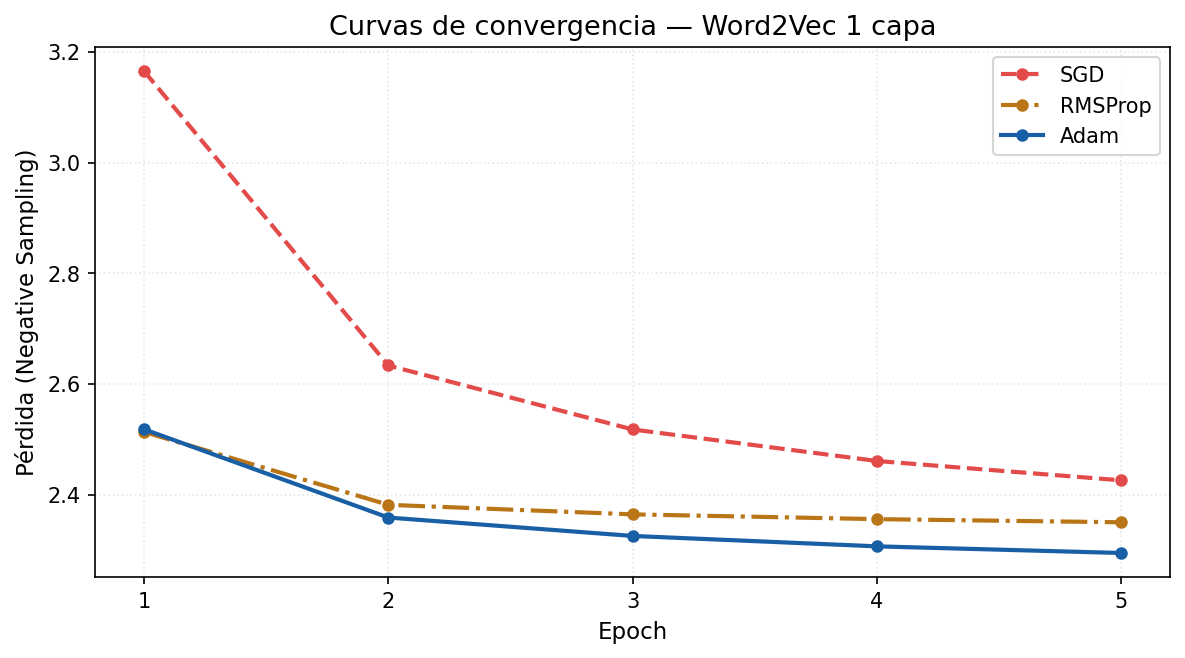
\includegraphics[width=0.72\textwidth]{convergencia_1_capa.png}
\caption{Curvas de convergencia --- Word2Vec de 1 capa oculta.}\label{fig:conv1}
\end{figure}
\begin{figure}[H]
\centering
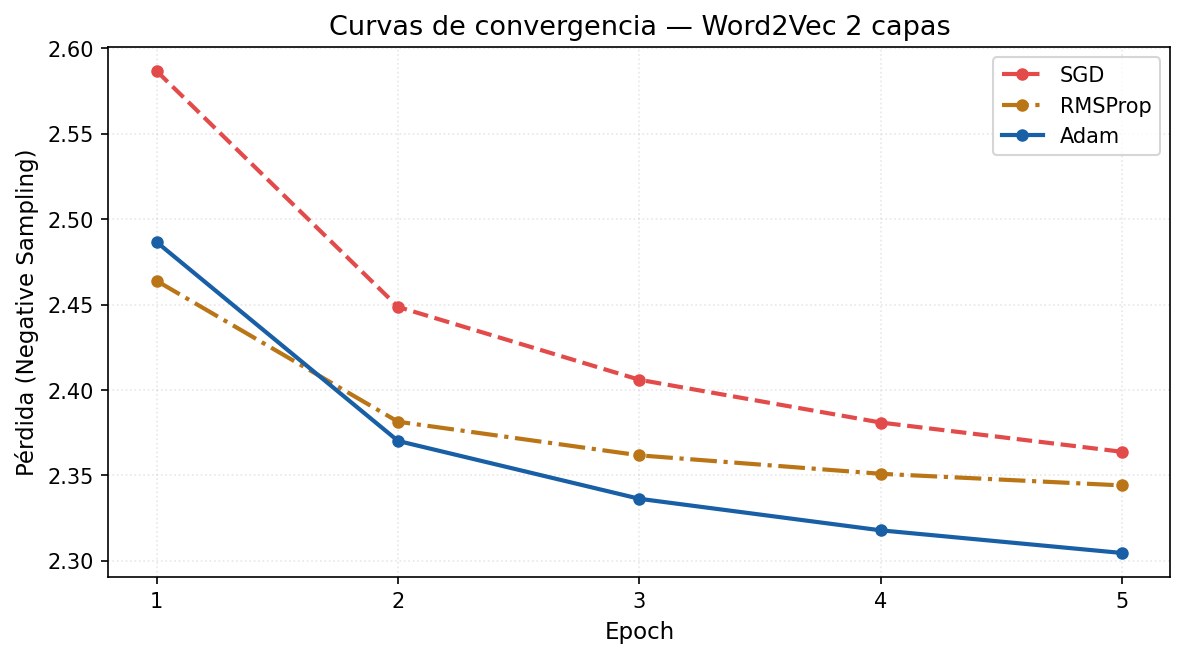
\includegraphics[width=0.72\textwidth]{convergencia_2_capas.png}
\caption{Curvas de convergencia --- Word2Vec de 2 capas ocultas.}\label{fig:conv2}
\end{figure}

\subsection{Resultados de clasificación}
El Cuadro~\ref{tab:main} resume F1-macro y Accuracy en test para las seis configuraciones,
cada optimizador con su tasa estable.
\begin{table}[H]
\centering
\caption{Clasificación en test (4\,000 muestras). Cada optimizador con su $\eta$ estable.}
\label{tab:main}
\begin{tabular}{llcccc}
\toprule
Arquitectura & Optimizador & $\eta$ & Accuracy & F1-macro & Tiempo (s) \\
\midrule
1 capa  & SGD     & 0.1   & 0.8608 & 0.8607 & 221 \\
1 capa  & RMSProp & 0.001 & 0.8940 & \textbf{0.8940} & 183 \\
1 capa  & Adam    & 0.001 & 0.8932 & 0.8932 & 188 \\
2 capas & SGD     & 0.1   & 0.8812 & 0.8812 & 302 \\
2 capas & RMSProp & 0.001 & 0.8822 & 0.8822 & 181 \\
2 capas & Adam    & 0.001 & 0.8900 & 0.8900 & 198 \\
\bottomrule
\end{tabular}
\end{table}

\subsection{Visualización de embeddings}
La Figura~\ref{fig:tsne} muestra una proyección t-SNE de los embeddings más frecuentes
(1 capa, Adam): palabras semánticamente relacionadas quedan próximas, evidenciando estructura
semántica capturada del corpus.
\begin{figure}[H]
\centering
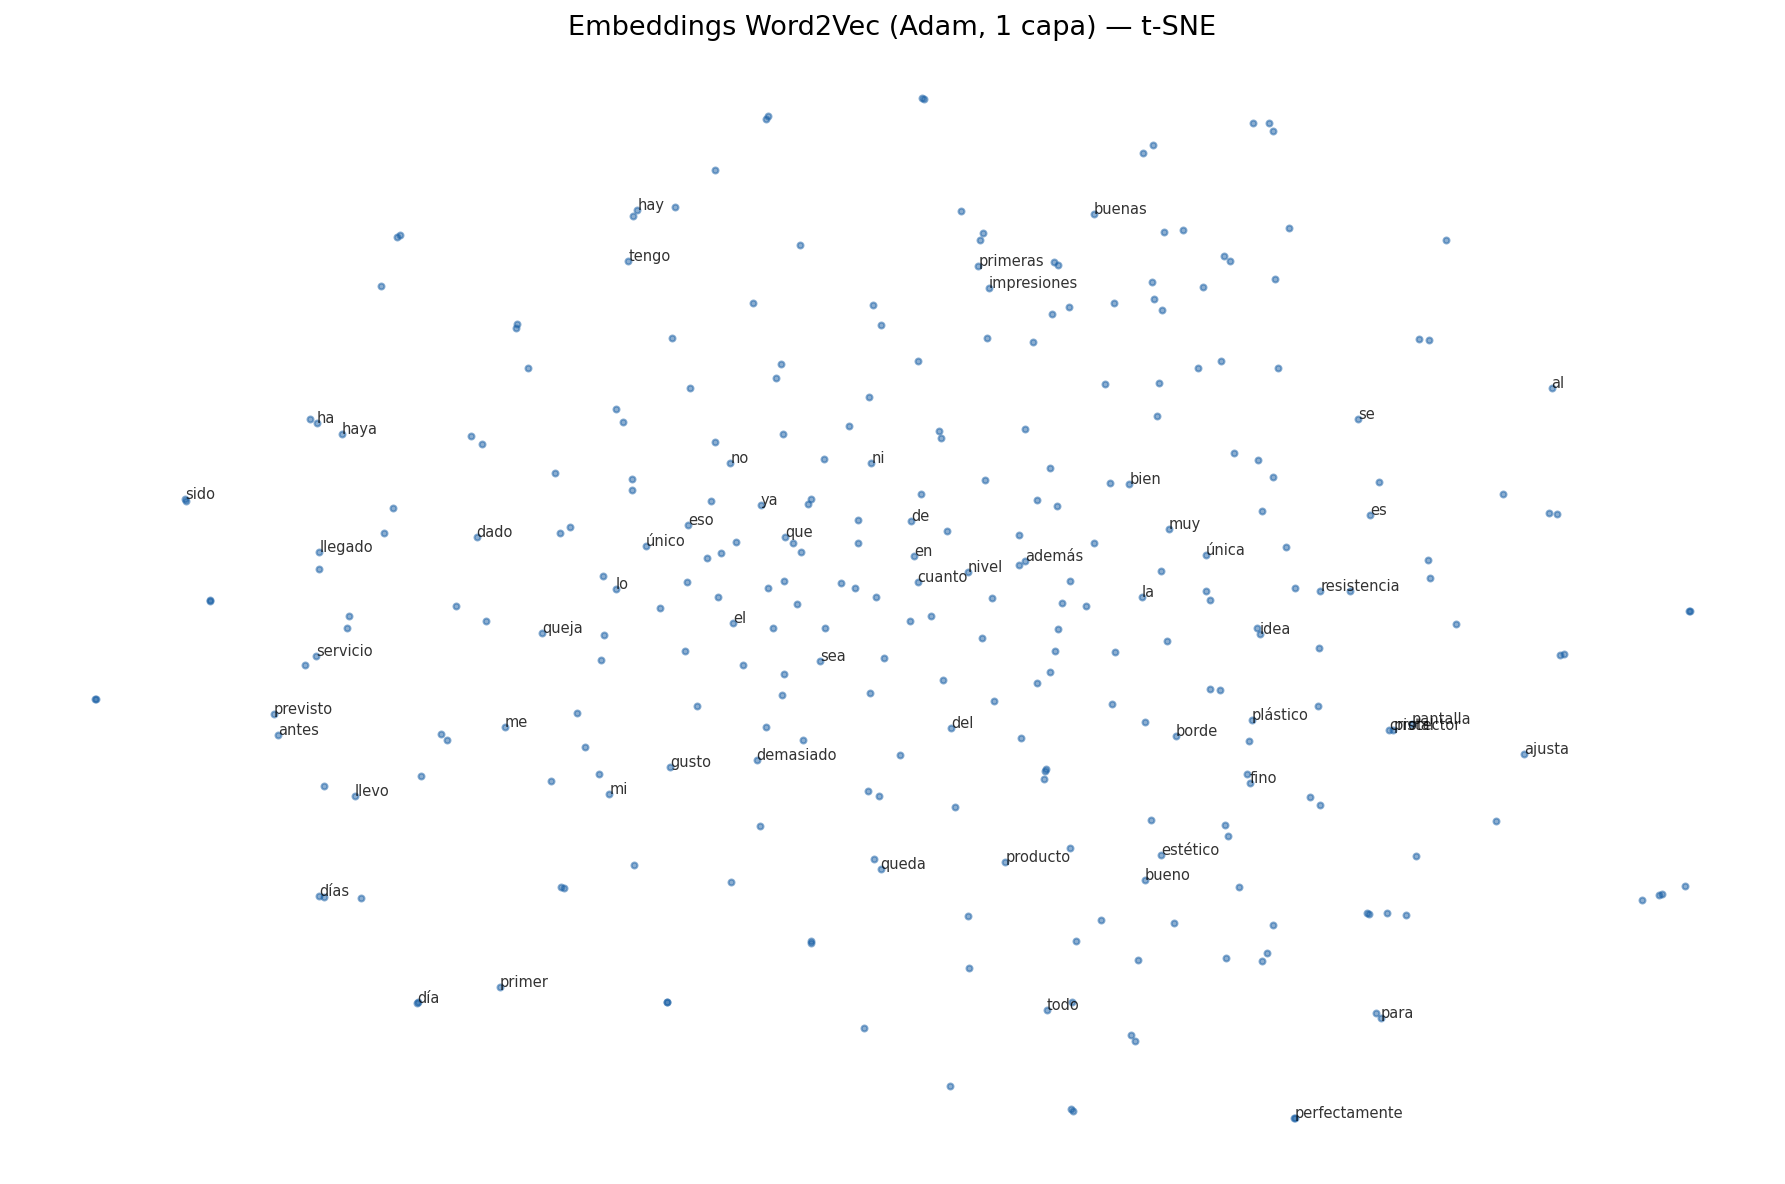
\includegraphics[width=0.7\textwidth]{tsne_embeddings.png}
\caption{Proyección t-SNE de embeddings Word2Vec (1 capa, Adam).}\label{fig:tsne}
\end{figure}

\subsection{Experimento 1: Sensibilidad de SGD al learning rate}
La Figura~\ref{fig:exp1} y el Cuadro~\ref{tab:exp1} muestran el comportamiento de SGD según
$\eta$. La sensibilidad es dramática: el mismo algoritmo pasa de F1$=0.87$ a F1$=0.62$ según
la tasa.
\begin{figure}[H]
\centering
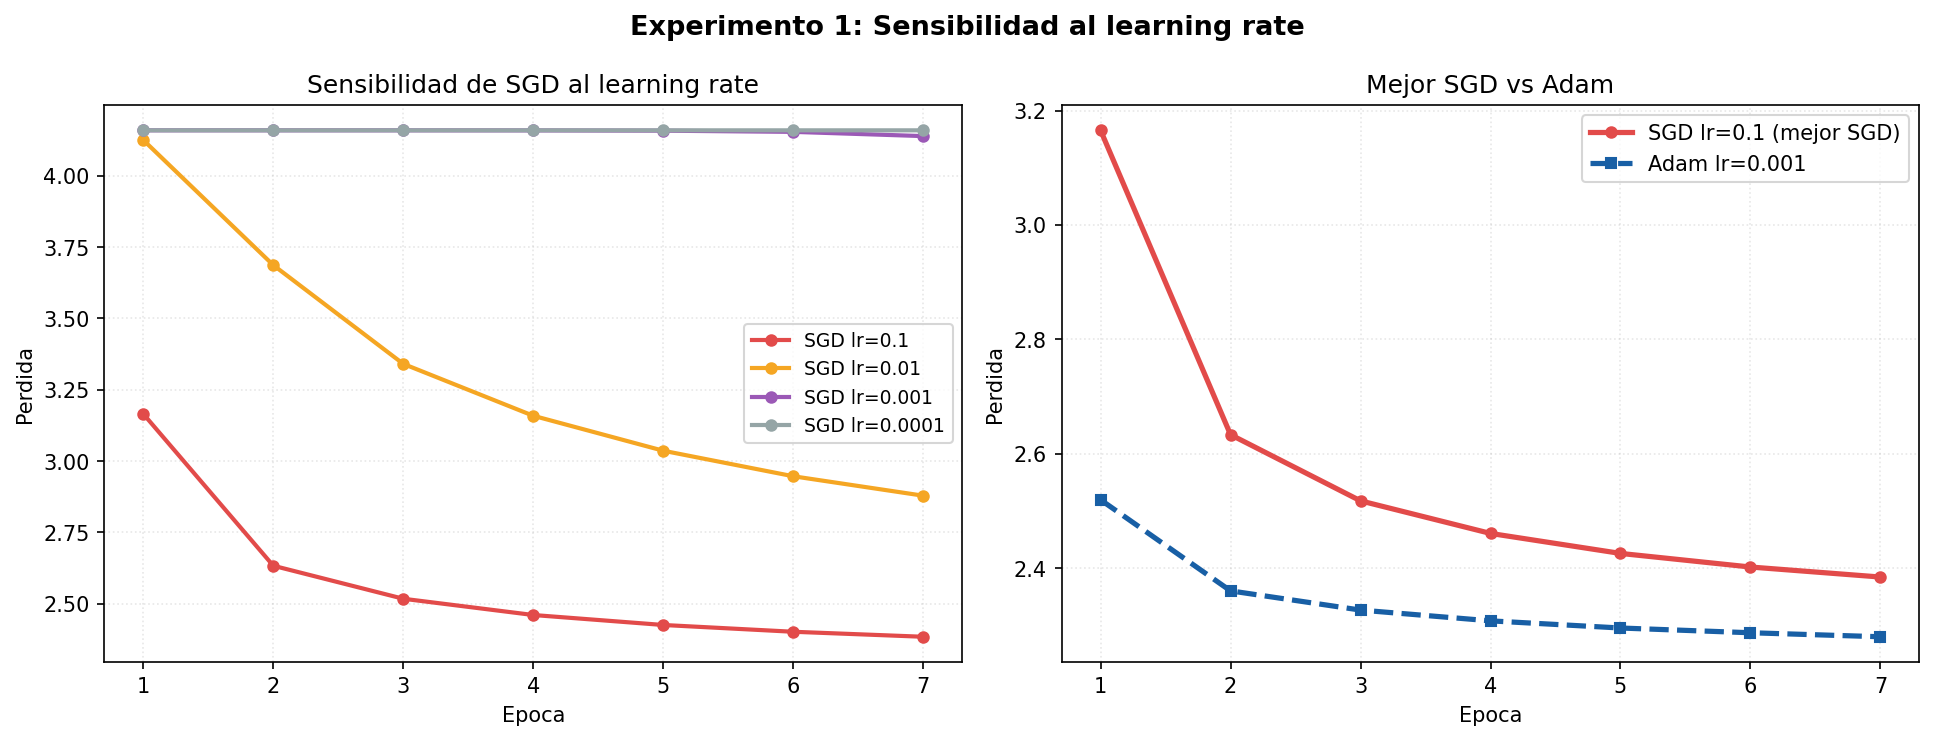
\includegraphics[width=0.85\textwidth]{exp1_lr_sensitivity.png}
\caption{Izq.: pérdida de SGD para cuatro tasas. Der.: mejor SGD ($\eta=0.1$) vs.\ Adam.}
\label{fig:exp1}
\end{figure}
\begin{table}[H]
\centering
\caption{SGD según learning rate (1 capa, 7 épocas).}\label{tab:exp1}
\begin{tabular}{lccl}
\toprule
Learning rate & F1-macro & Pérdida final & Comportamiento \\
\midrule
$\eta=0.1$    & \textbf{0.8742} & 2.384 & Converge bien \\
$\eta=0.01$   & 0.7715 & 2.879 & Converge lento \\
$\eta=0.001$  & 0.6212 & 4.139 & Estancado \\
$\eta=0.0001$ & 0.6829 & 4.159 & Congelado \\
\bottomrule
\end{tabular}
\end{table}

\subsection{Experimento 2: Tracking de la norma del gradiente}
La Figura~\ref{fig:exp2} registra la pérdida y la norma promedio del gradiente $\|\nabla L\|$
por época para SGD y Adam, \emph{ambos con $\eta=0.001$}. A esa tasa, SGD permanece en la
meseta de inicialización (pérdida $\approx 4.14$) con un gradiente $\sim$80$\times$ menor que
el de Adam en la primera época ($0.0016$ vs.\ $0.1305$); la razón decae a $\sim$7$\times$ en
la época~7 a medida que SGD empieza a moverse muy lentamente. El mecanismo es claro: Adam
\emph{normaliza} el gradiente por su historia acumulada, dando pasos efectivos de magnitud
útil donde SGD da pasos despreciables.
\begin{figure}[H]
\centering
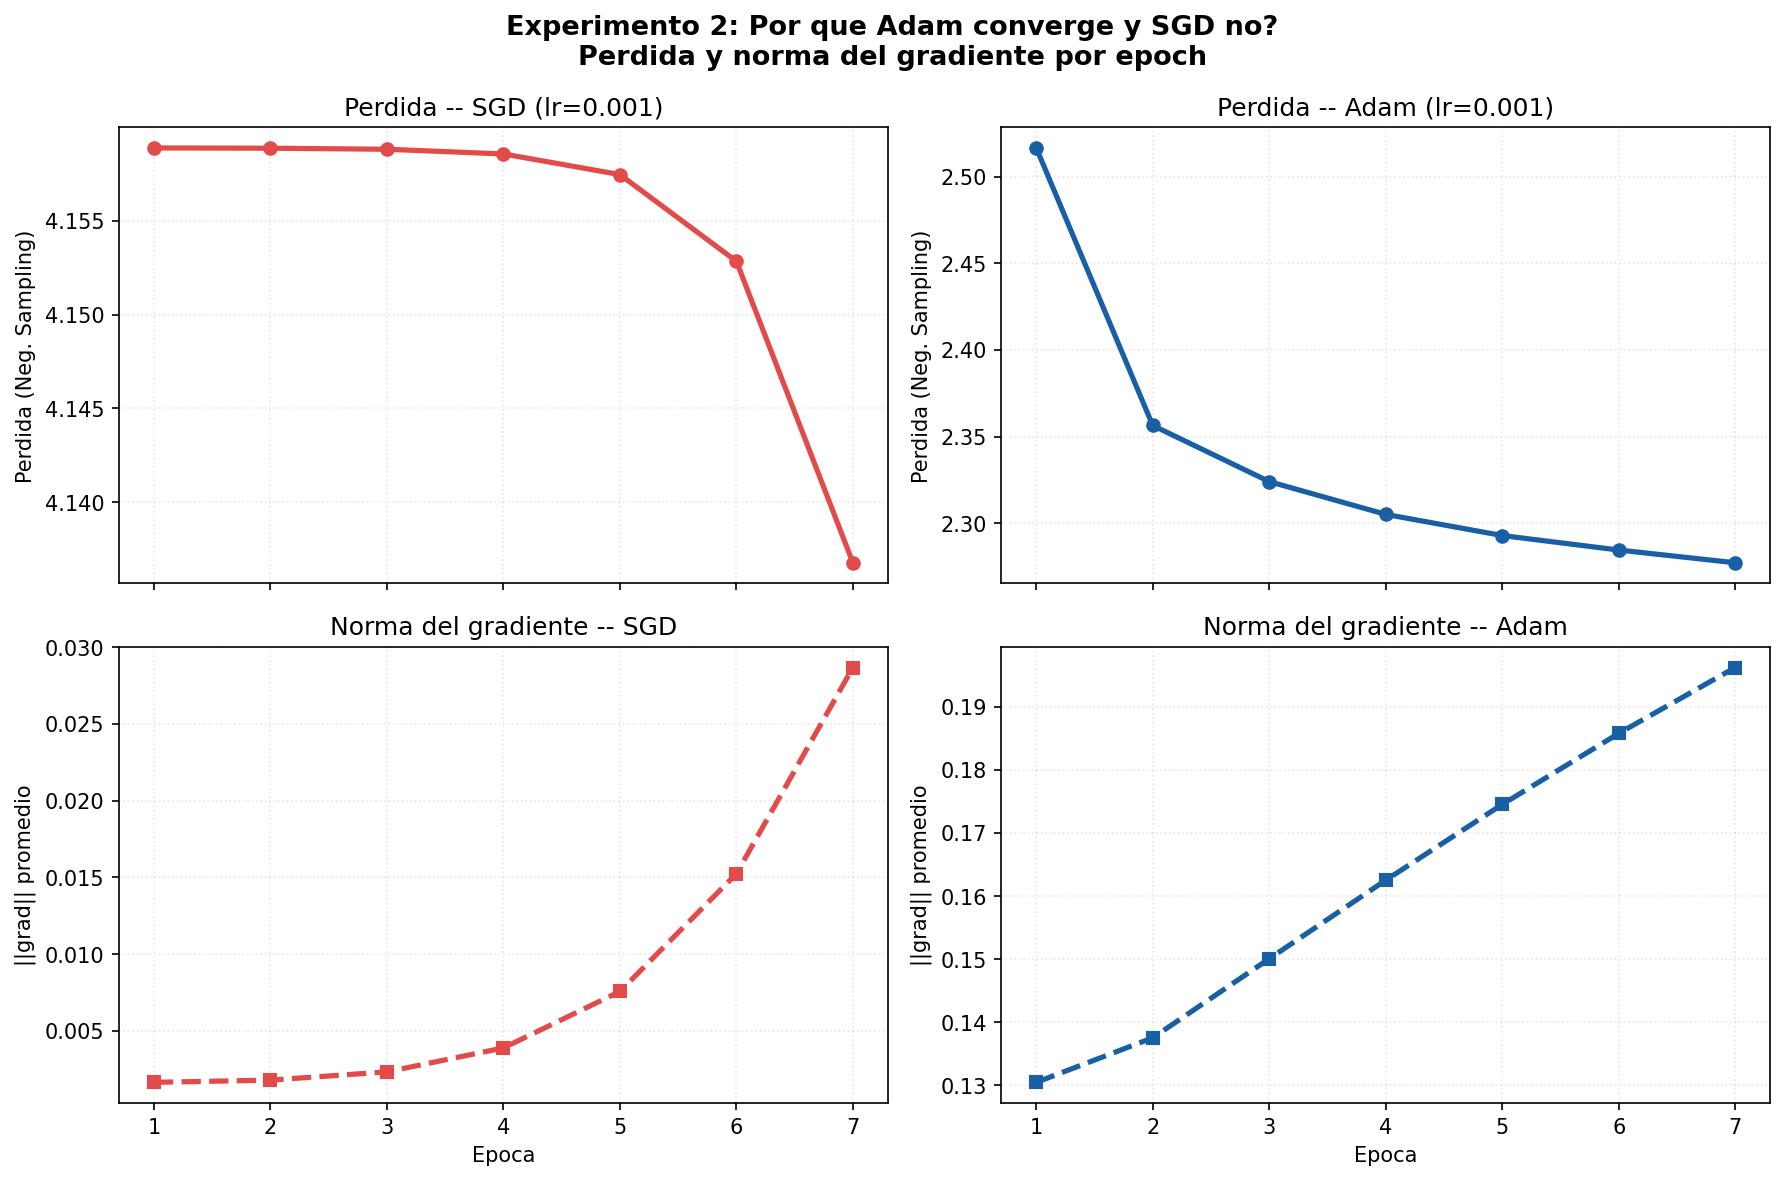
\includegraphics[width=0.85\textwidth]{exp2_grad_tracking.png}
\caption{Pérdida y norma del gradiente para SGD y Adam ($\eta=0.001$).}\label{fig:exp2}
\end{figure}

\subsection{Experimento 3: Baseline TF-IDF y ablación de dimensión}
El Cuadro~\ref{tab:exp3} compara Word2Vec contra TF-IDF y varía $d$. Crucialmente,
\textbf{incluso TF-IDF con solo unigramas} ($0.9107$) supera al mejor Word2Vec; con bigramas
sube a $0.9225$.
\begin{figure}[H]
\centering
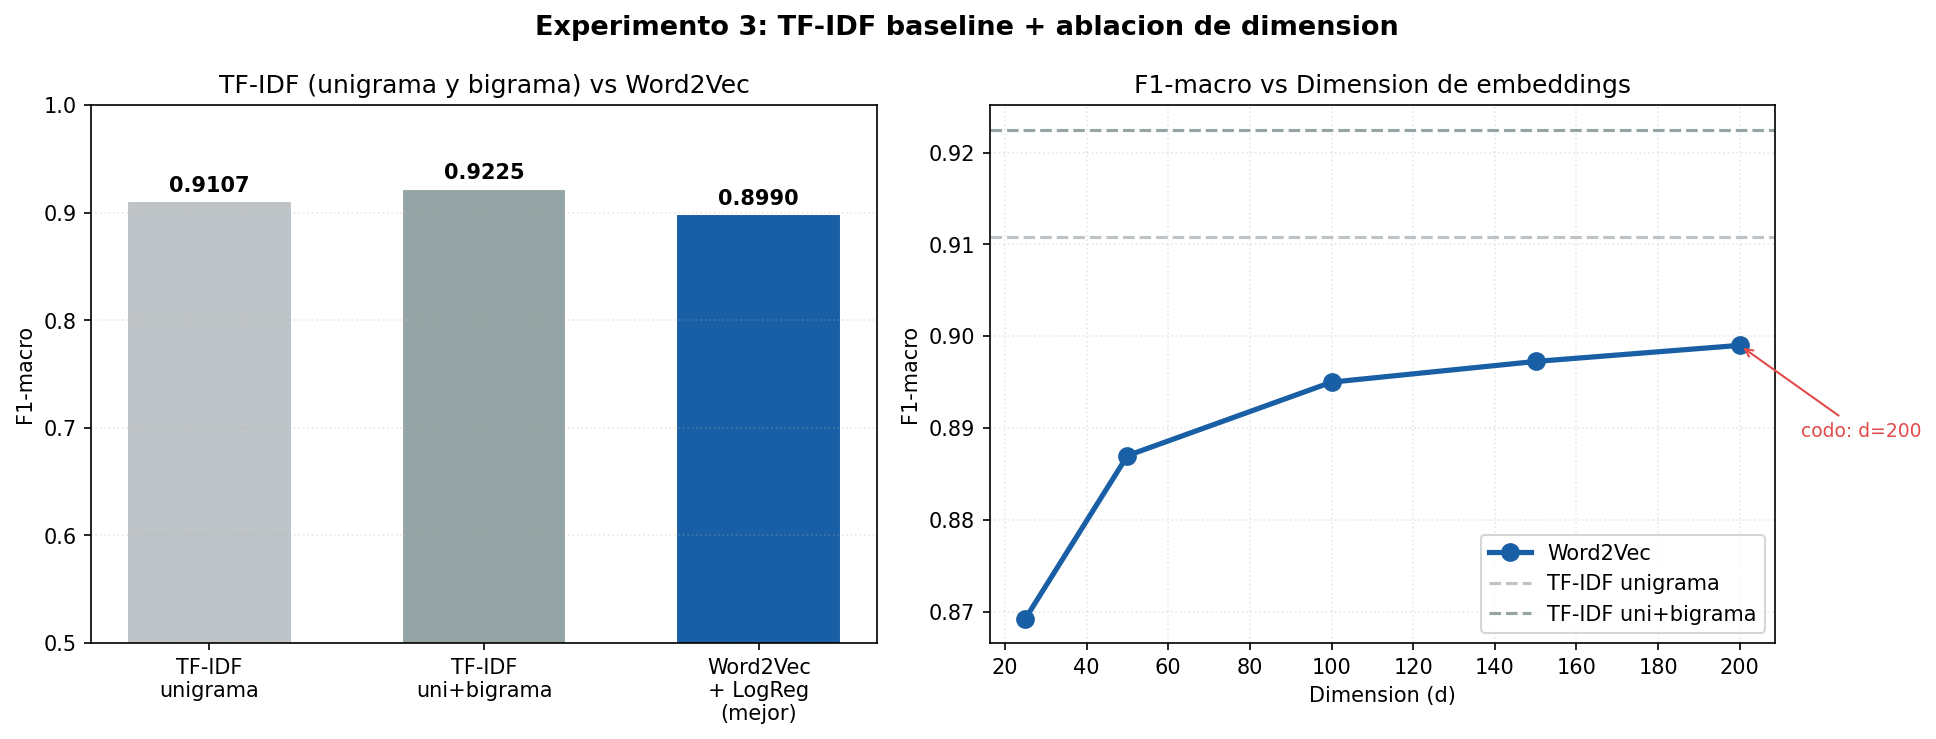
\includegraphics[width=0.85\textwidth]{exp3_tfidf_ablacion.png}
\caption{Izq.: TF-IDF (unigrama y bigrama) vs.\ Word2Vec. Der.: F1 en función de $d$.}
\label{fig:exp3}
\end{figure}
\begin{table}[H]
\centering
\caption{Ablación de dimensión (Adam, 5 épocas) y baseline TF-IDF.}\label{tab:exp3}
\begin{tabular}{lc}
\toprule
Representación & F1-macro \\
\midrule
Word2Vec $d=25$  & 0.8692 \\
Word2Vec $d=50$  & 0.8870 \\
Word2Vec $d=100$ & 0.8950 \\
Word2Vec $d=150$ & 0.8972 \\
Word2Vec $d=200$ & 0.8990 \\
\midrule
TF-IDF unigrama (1,1) & 0.9107 \\
TF-IDF uni+bigrama (1,2) & \textbf{0.9225} \\
\bottomrule
\end{tabular}
\end{table}

\subsection{Experimento 4: Análisis semántico}
El Cuadro~\ref{tab:exp4} muestra los vecinos por similitud coseno: son semánticamente
coherentes (incluyendo sinónimos y faltas ortográficas del corpus), lo que evidencia
interpretabilidad directa de los parámetros aprendidos. Las 15 palabras de consulta se
encontraron en el vocabulario (15/15).
\begin{table}[H]
\centering
\caption{Top-5 palabras más similares por similitud coseno (Adam, $d=100$).}\label{tab:exp4}
\begin{tabular}{ll}
\toprule
Consulta & Vecinos (similitud coseno) \\
\midrule
excelente  & inmejorable (0.79), exelente (0.76), buenisimo (0.75), excepcional (0.74) \\
horrible   & fatal (0.72), pésimo (0.66), malísimo (0.62), desastre (0.57) \\
roto       & doblado (0.76), rajado (0.75), estropeado (0.73), destrozado (0.72) \\
recomiendo & aconsejo (0.77), recomendaría (0.70), recomendaria (0.69), volvería (0.64) \\
envio      & envío (0.84), envió (0.80), entrega (0.70), estimado (0.69) \\
\bottomrule
\end{tabular}
\end{table}
\begin{figure}[H]
\centering
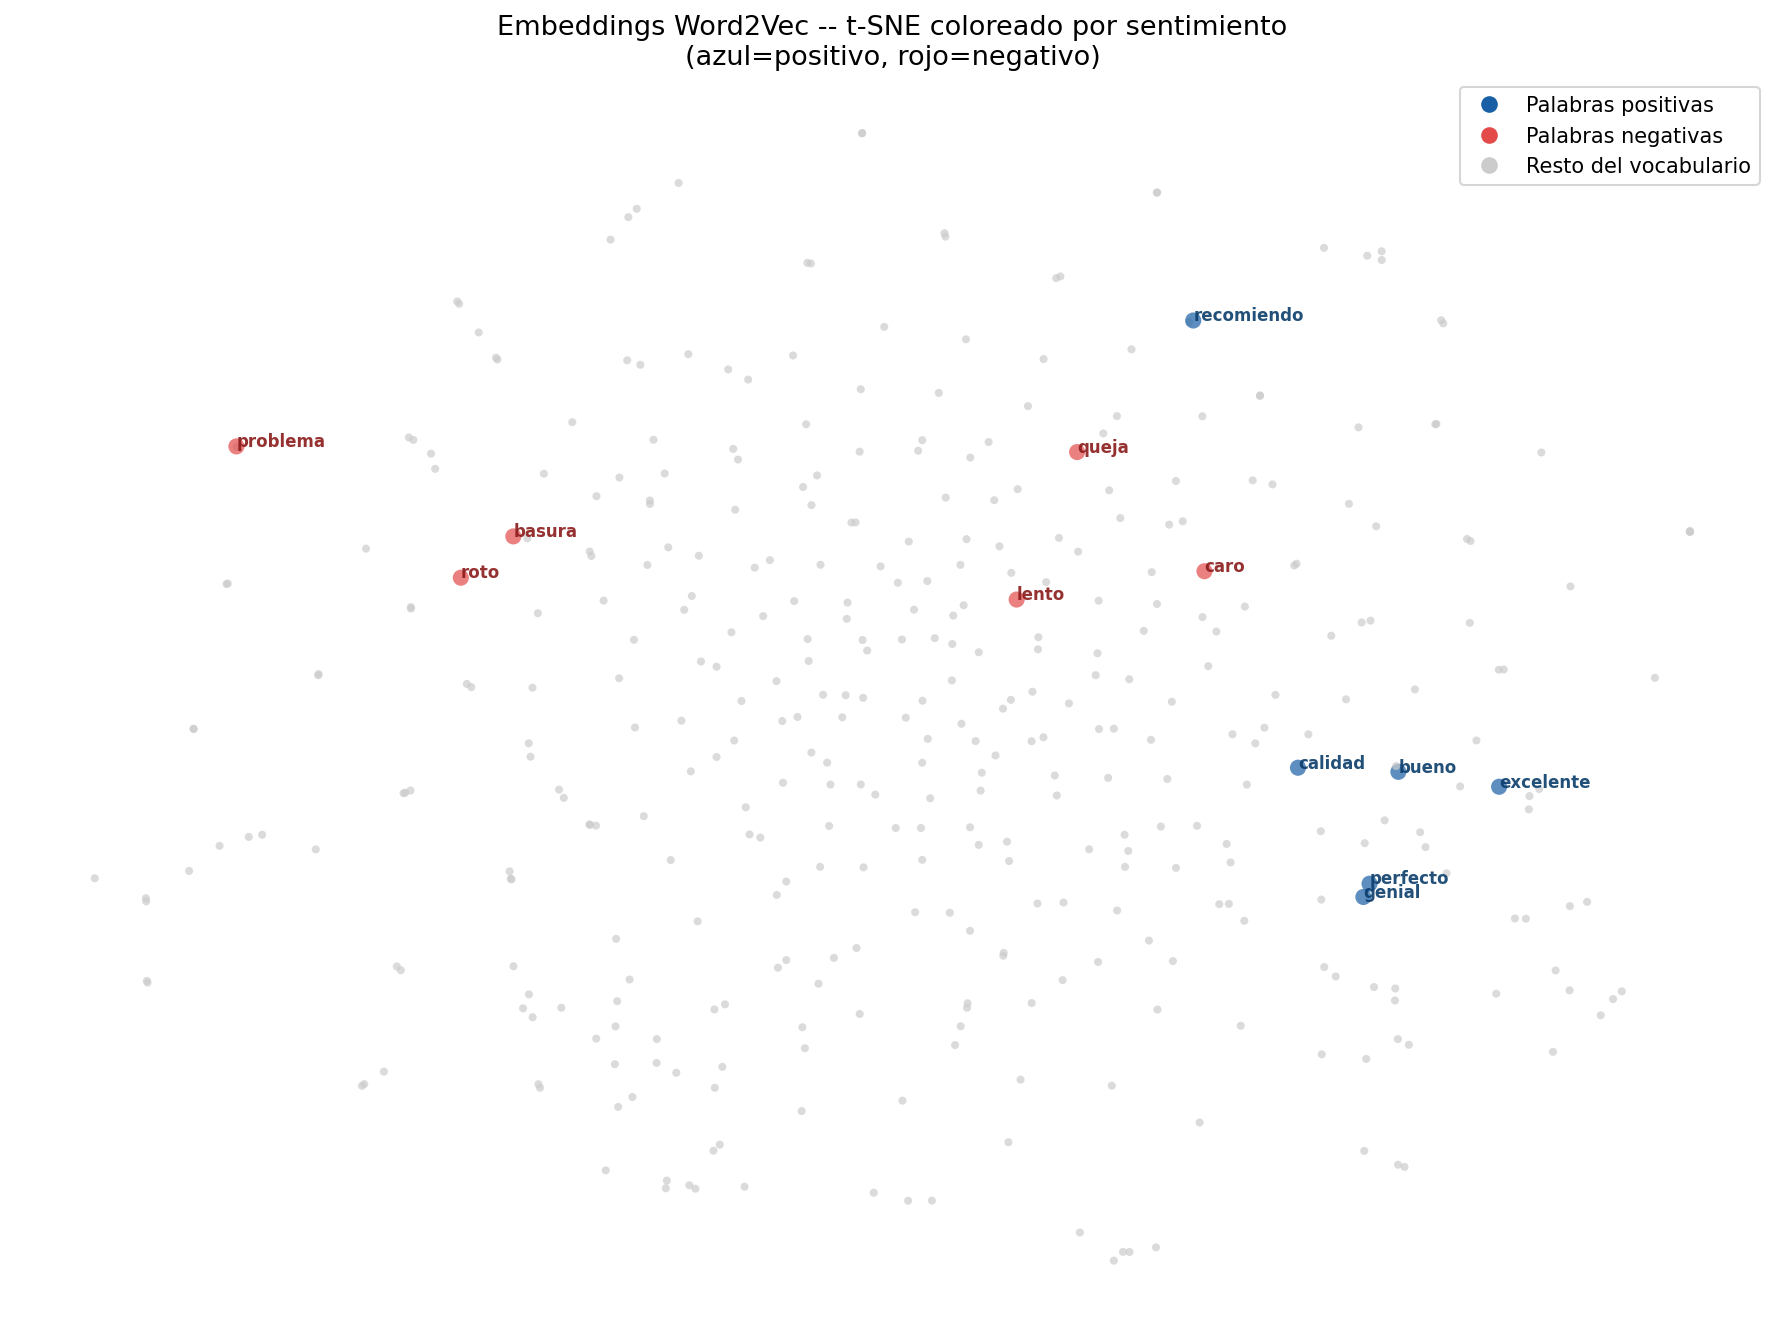
\includegraphics[width=0.7\textwidth]{exp4_tsne_colored.png}
\caption{t-SNE coloreado por polaridad: azul = positivas, rojo = negativas.}\label{fig:exp4}
\end{figure}

\subsection{Experimentos 5 y 5b: Búsqueda de hiperparámetros}
El grid (5 tasas $\times$ 4 dimensiones) y la búsqueda Bayesiana (Optuna TPE, 30 trials)
convergen a la misma región y dan F1-test prácticamente idéntico (Cuadro~\ref{tab:exp5}).
Notablemente, el óptimo del grid queda en el \emph{interior} del espacio explorado (peor por
encima y por debajo), por lo que el rango de búsqueda fue adecuado.
\begin{figure}[H]
\centering
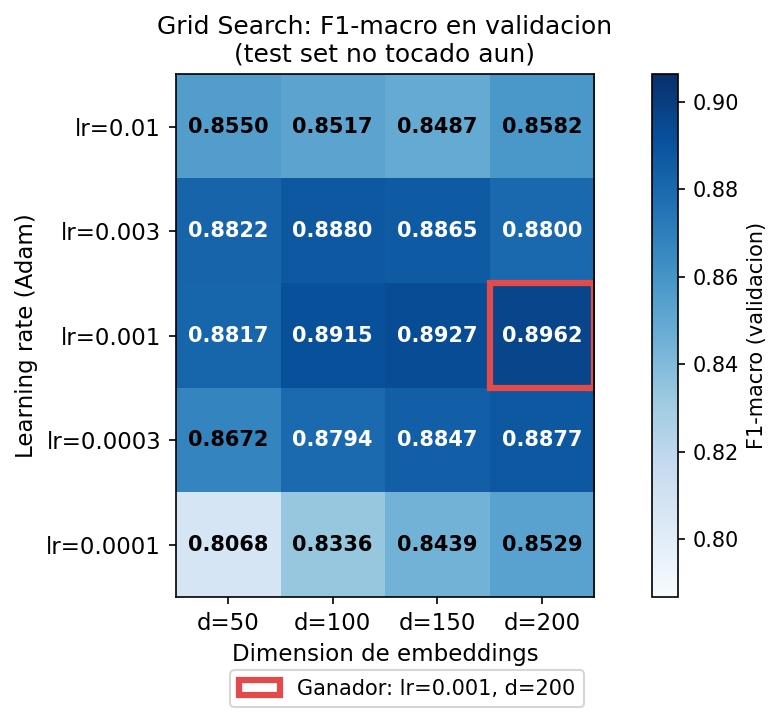
\includegraphics[width=0.6\textwidth]{exp5_grid_heatmap.png}
\caption{Heatmap de F1-validación del grid search. El óptimo ($\eta=0.001$, $d=200$) es
interior.}\label{fig:exp5}
\end{figure}
\begin{table}[H]
\centering
\caption{Grid search vs.\ búsqueda Bayesiana.}\label{tab:exp5}
\begin{tabular}{lccc}
\toprule
Método & Config.\ óptima & F1-val & F1-test \\
\midrule
Grid search   & $\eta=0.001$, $d=200$    & 0.8962 & 0.8972 \\
Optuna (TPE)  & $\eta=0.00059$, $d=166$  & 0.8980 & 0.8970 \\
\bottomrule
\end{tabular}
\end{table}

\subsection{Experimento 6: Duelo contra SBWC preentrenado}\label{sec:exp6}
Una vez optimizado nuestro modelo, lo enfrentamos a los embeddings preentrenados
\textbf{SBWC} (Spanish Billion Word Corpus, $\sim$1.5\,B palabras, 300d). Para una comparación
justa, ambos usan el mismo clasificador y preprocesamiento; solo cambia la matriz de
embeddings. Se mide F1-macro en tres escenarios: \emph{Amazon} (in-domain), \emph{Tweets}
transferencia (clasificador entrenado en Amazon y probado en tweets) y \emph{Tweets}
in-domain (clasificador entrenado sobre un split de tweets). El dataset out-of-domain son
tweets en español de CardiffNLP~\cite{barbieri2022}.
\begin{table}[H]
\centering
\caption{Duelo de embeddings (F1-macro). Clasificador y preprocesamiento idénticos.}
\label{tab:exp6}
\begin{tabular}{lccc}
\toprule
Representación & Amazon (in-dom.) & Tweets (transf.) & Tweets (in-dom.) \\
\midrule
Nuestro W2V ($d=300$) & \textbf{0.9027} & 0.6733 & 0.7129 \\
SBWC preentrenado     & 0.8830 & \textbf{0.7529} & \textbf{0.7589} \\
TF-IDF (referencia)   & 0.9225 & 0.6829 & 0.7222 \\
\bottomrule
\end{tabular}
\end{table}
La cobertura de vocabulario en los tweets es de \textbf{82.7\%} para nuestro modelo y
\textbf{96.4\%} para SBWC (Figura~\ref{fig:exp6}). Dos lecturas:
\begin{enumerate}
  \item \textbf{En su propio dominio, nuestro modelo de 40\,k reseñas supera al gigante de
  1.5\,B palabras} (0.903 vs.\ 0.883): el entrenamiento in-domain captura el léxico
  específico de reseñas de productos.
  \item \textbf{Fuera de dominio, SBWC generaliza mejor} (0.759 vs.\ 0.713 in-domain sobre
  tweets). La variante in-domain confirma que la diferencia \emph{no} es solo desajuste del
  clasificador, sino calidad de representación: aun entrenando el clasificador sobre tweets,
  nuestro modelo choca con un techo impuesto por su vocabulario cerrado (82.7\% de cobertura).
\end{enumerate}
\begin{figure}[H]
\centering
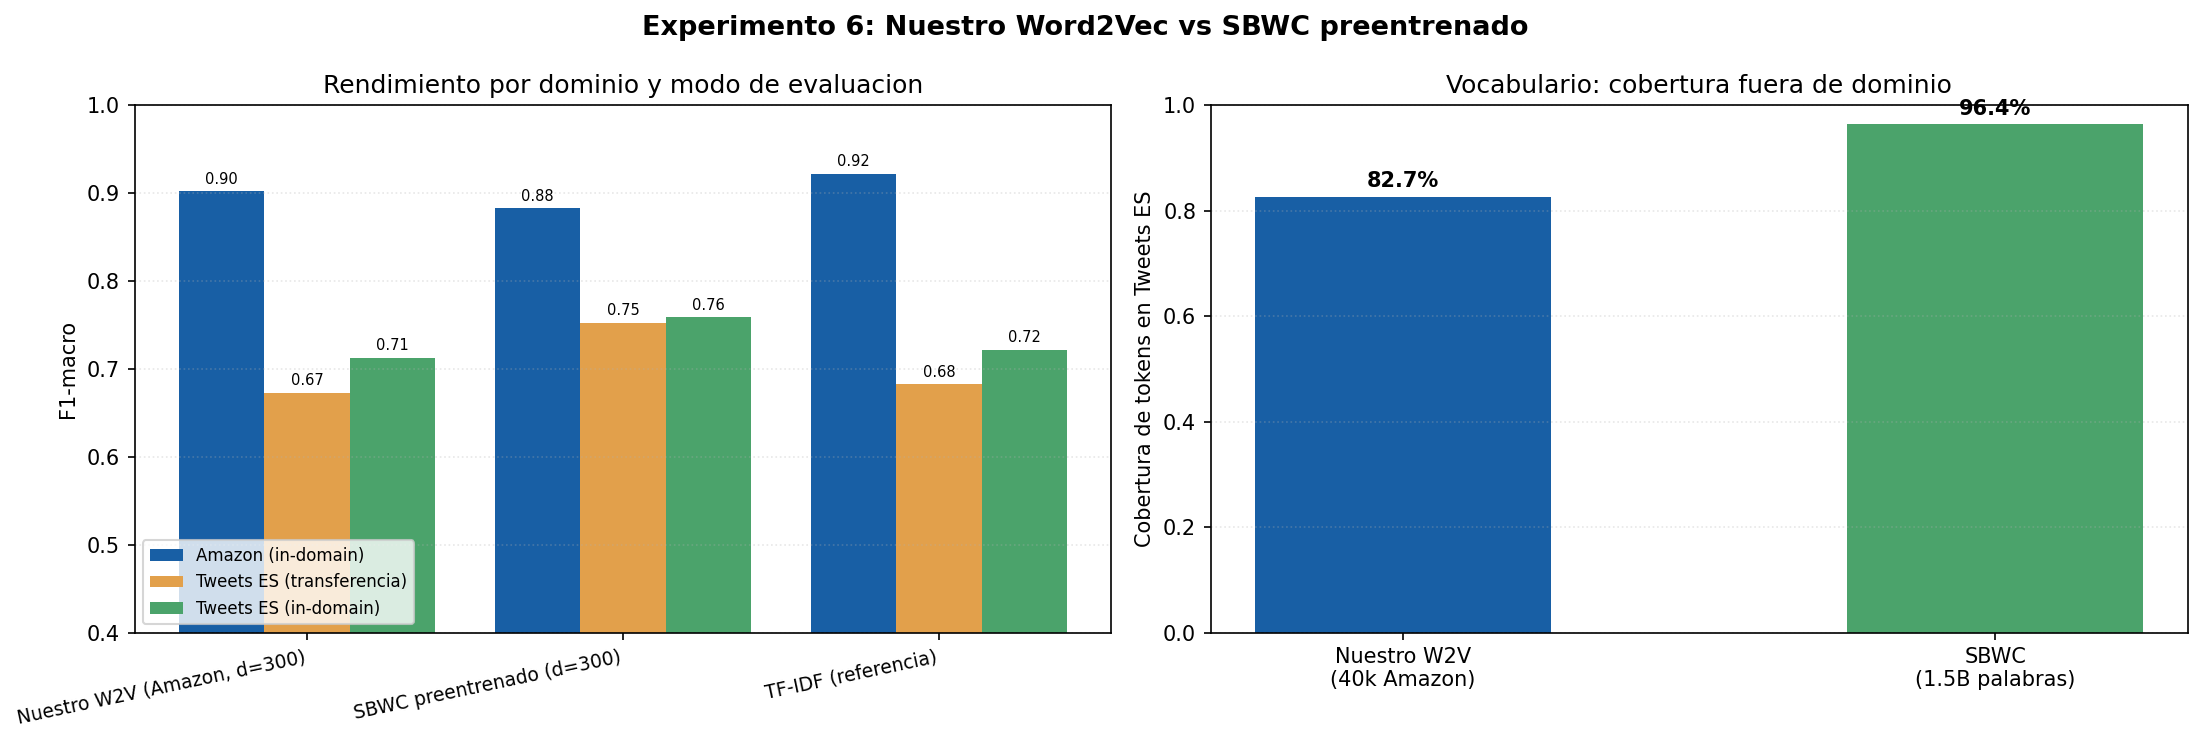
\includegraphics[width=\textwidth]{exp6_duelo_sbwc.png}
\caption{Duelo W2V vs.\ SBWC: rendimiento por dominio (izq.) y cobertura de vocabulario
fuera de dominio (der.).}\label{fig:exp6}
\end{figure}

\subsection{Verificación del gradiente analítico}\label{sec:gradcheck}
Para cerrar el círculo entre la teoría y la práctica del descenso del gradiente, se verifica
que el gradiente derivado a mano (Ecuación~\eqref{eq:grad}) es correcto. Se compara contra:
(A) la diferenciación automática de PyTorch y (B) un gradiente numérico por diferencias
finitas en doble precisión. Las tres coinciden: el error máximo entre la fórmula analítica y
autograd es del orden de $10^{-16}$, y la prueba de diferencias finitas
(\texttt{torch.autograd.gradcheck}) pasa. Esto confirma que la implementación minimiza
exactamente la pérdida~\eqref{eq:ns} mediante su gradiente correcto.

% ============================================================
\section{Análisis y discusión}\label{sec:analisis}

\paragraph{H1 (confirmada, con matiz).} Con la \emph{misma} tasa $\eta=0.001$, los métodos
adaptativos superan ampliamente a SGD, que se estanca (exp2). Sin embargo, esto no significa
que SGD sea un algoritmo inferior: con su propia tasa ($\eta=0.1$) alcanza F1$=0.861$, a solo
$\sim$3 puntos del mejor adaptativo. La diferencia es de \emph{ajuste}, no de calidad
intrínseca.

\paragraph{H3 (confirmada).} SGD es brutalmente sensible al \emph{learning rate}: barre de
F1$=0.62$ a F1$=0.87$ según $\eta$ (exp1), mientras Adam opera bien en un rango amplio. El
mecanismo lo explica exp2: la inicialización de la matriz de salida en ceros crea una meseta
casi plana; el momentum y, sobre todo, la normalización adaptativa permiten escapar de ella,
cosa que SGD a tasa pequeña no logra.

\paragraph{H2 (refutada, con matiz).} La arquitectura de 2 capas no supera a la de 1 capa: el
mejor modelo es 1 capa + RMSProp (0.8940) frente al mejor de 2 capas (Adam, 0.8900). El
promedio de embeddings como vector de documento puede no aprovechar la transformación extra.
Curiosamente, la segunda capa \emph{sí} ayuda al optimizador débil (SGD pasa de 0.861 a
0.881): la no linealidad cambia el paisaje de pérdida de forma que favorece a SGD, aunque no
al mejor modelo global.

\paragraph{H4 (refutada).} El resultado más instructivo: TF-IDF supera a Word2Vec, y lo hace
\emph{incluso en su variante unigrama} (0.9107 vs.\ 0.8990), descartando que la ventaja se
deba solo a los bigramas. Refleja una propiedad del dominio: las reseñas de Amazon tienen
vocabulario directo y discriminativo (``excelente'', ``pésimo'', ``no funciona''), donde la
presencia o ausencia de palabras clave basta para clasificar. Word2Vec destaca en dominios
donde el contexto importa más que las palabras aisladas --- lo que se confirma fuera de
dominio (Sección~\ref{sec:exp6}).

\paragraph{H5 (refutada).} La búsqueda Bayesiana (Optuna, 30 trials, espacio continuo)
encontró $\eta^{*}=0.00059$, $d^{*}=166$ con F1-test$=0.8970$, prácticamente idéntico al grid
($0.8972$). El óptimo del grid es \emph{interior} al espacio explorado, lo que indica que el
paisaje de validación es plano alrededor del óptimo y que una rejilla bien diseñada es más
costo-efectiva que la búsqueda Bayesiana en este problema.

\paragraph{H6 (confirmada, con matiz importante).} SBWC generaliza mejor fuera de dominio
(0.759 vs.\ 0.713 en tweets), validado por la cobertura de vocabulario (96.4\% vs.\ 82.7\%).
Pero la dirección se \emph{invierte} en dominio: nuestro modelo entrenado in-domain supera a
SBWC en Amazon (0.903 vs.\ 0.883). La conclusión no es ``el preentrenado es mejor'', sino un
\emph{trade-off de dominio}: representaciones específicas ganan en casa, representaciones
generales ganan al transferir.

\paragraph{Interpretabilidad de los parámetros.} El exp4 verifica que los embeddings tienen
semántica real (excelente $\to$ inmejorable, roto $\to$ doblado, recomiendo $\to$ aconsejo).
Esta interpretabilidad directa de la matriz $W_{in}$ es una ventaja clave frente a modelos
más complejos.

\paragraph{Nota sobre el diseño experimental.} Algunas elecciones merecen justificación
explícita: (i) cada optimizador usa su tasa estable para una comparación justa; (ii) exp1 y
exp2 usan 7 épocas (en vez de 5) para dar resolución a la dinámica lenta de SGD; (iii) los
experimentos de afinación usan Adam, indistinguible de RMSProp ($<0.001$ de F1) y estándar de
facto; (iv) el duelo usa $d=300$ para igualar la dimensión de SBWC, dentro de la meseta de
rendimiento ($d\gtrsim 150$).

% ============================================================
\section{Fortalezas, limitaciones y usos profesionales}

\subsection{Fortalezas}
\textbf{Eficiencia y compacidad:} Word2Vec representa cada documento con 300 números densos y
queda a 1--2 puntos de un TF-IDF de 50\,000 features. \textbf{Transferibilidad:} los
embeddings se reutilizan en otras tareas, como evidencia el duelo fuera de dominio.
\textbf{Interpretabilidad:} distancia $=$ similitud semántica (exp4). \textbf{Auto-supervisión:}
se entrena sin etiquetas.

\subsection{Limitaciones}
\textbf{Embeddings estáticos:} ``banco'' (financiero/mueble) tiene un solo vector.
\textbf{Vocabulario cerrado:} las palabras no vistas no tienen representación --- cuantificado
en el exp6 (82.7\% de cobertura fuera de dominio, frente al 96.4\% de SBWC).
\textbf{Promedio de documento:} pierde el orden de las palabras.

\subsection{Usos actuales en el ámbito profesional}
Word2Vec y sus variantes se usan en: motores de recomendación (representando ítems como
``palabras'' en secuencias de interacción), búsqueda semántica y \emph{retrieval}, análisis
de sentimiento y \emph{routing} en atención al cliente, expansión de consultas, y como
inicialización de embeddings en modelos más complejos. Su bajo costo y su transferibilidad lo
mantienen vigente como baseline fuerte y como componente de sistemas de producción donde la
latencia y la interpretabilidad importan.

% ============================================================
\section{Conclusiones}\label{sec:conclusiones}
\begin{enumerate}
  \item \textbf{H1 confirmada:} a igual tasa ($\eta=0.001$), Adam y RMSProp convergen y SGD se
  estanca (gradiente $\sim$80$\times$ menor); pero con su tasa ($\eta=0.1$) SGD alcanza
  F1$=0.861$. La sensibilidad al \emph{learning rate}, no la calidad intrínseca, es el factor
  determinante.
  \item \textbf{H2 refutada:} la segunda capa no mejora la clasificación final. El mejor
  modelo es Word2Vec de 1 capa con RMSProp (F1$=0.8940$).
  \item \textbf{H3 confirmada:} SGD requiere ajuste fino de $\eta$ (F1 de 0.62 a 0.87);
  Adam es robusto.
  \item \textbf{H4 refutada:} TF-IDF supera a Word2Vec incluso con unigramas (0.9107 vs.\
  0.8990); el vocabulario directo del corpus favorece las representaciones dispersas.
  \item \textbf{H5 refutada:} la búsqueda Bayesiana no mejora significativamente al grid
  ($\Delta$F1-test $<0.001$); el óptimo es interior y el paisaje, plano.
  \item \textbf{H6 confirmada con matiz:} SBWC generaliza mejor fuera de dominio (cobertura
  96.4\% vs.\ 82.7\%), pero nuestro modelo in-domain lo supera en Amazon (0.903 vs.\ 0.883).
  Hay un trade-off de dominio, no un ganador absoluto.
  \item \textbf{Sobre el curso:} Word2Vec es un caso de estudio ideal de optimización ---
  permite ver la función de pérdida, derivar y \emph{verificar} su gradiente, comparar
  algoritmos de minimización y buscar hiperparámetros --- todo sobre un problema real de NLP
  en español.
\end{enumerate}

% ============================================================
\begin{thebibliography}{9}
\bibitem{harris1954} Z. S. Harris. \emph{Distributional structure}. Word, 10(2--3):146--162, 1954.
\bibitem{keung2020} P. Keung, Y. Lu, G. Szarvas, N. A. Smith. \emph{The Multilingual Amazon Reviews Corpus}. EMNLP, 2020.
\bibitem{kingma2014} D. P. Kingma, J. Ba. \emph{Adam: A Method for Stochastic Optimization}. arXiv:1412.6980, 2014.
\bibitem{mikolov2013a} T. Mikolov, K. Chen, G. Corrado, J. Dean. \emph{Efficient Estimation of Word Representations in Vector Space}. arXiv:1301.3781, 2013.
\bibitem{mikolov2013b} T. Mikolov, I. Sutskever, K. Chen, G. Corrado, J. Dean. \emph{Distributed Representations of Words and Phrases and their Compositionality}. NeurIPS, 2013.
\bibitem{muennighoff2023} N. Muennighoff, N. Tazi, L. Magne, N. Reimers. \emph{MTEB: Massive Text Embedding Benchmark}. arXiv:2210.07316, 2023.
\bibitem{barbieri2022} F. Barbieri, L. Espinosa Anke, J. Camacho-Collados. \emph{XLM-T: Multilingual Language Models in Twitter for Sentiment Analysis and Beyond}. LREC, 2022.
\end{thebibliography}

\end{document}
